\section{\large Исследовательская часть}

\subsection{Технические характеристики}

Тестирование выполнялось на устройстве со следующими техническими характеристиками:

\begin{itemize}
	\item Операционная система Pop!\_OS 22.04 LTS \cite{ubuntu} Linux \cite{linux};
	\item Оперативная память 32 Гбайт;
	\item Процессор AMD® Ryzen 7 2700 eight-core processor × 16 \cite{amd}.
\end{itemize}

\subsection{Демонстрация работы программы}

На рисунке \ref{TODO:risnok:1} представлен результат работы шифрования и время работы.

\begin{figure}[ht!]
	\centering{
		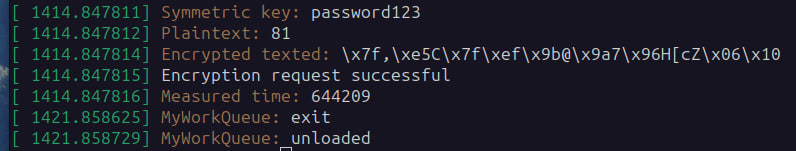
\includegraphics[width=0.5\textwidth]{assets/images/crypted.jpg}
		\caption{Результат работы с шифрованием}
		\label{TODO:risnok:1}}
\end{figure}

На рисунке \ref{TODO:risnok:2} представлен результат работы без шифрования и время работы.


\begin{figure}[ht!]
	\centering{
		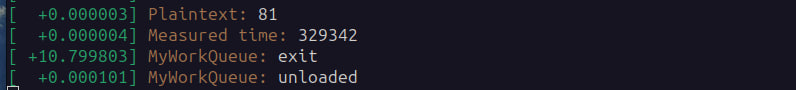
\includegraphics[width=0.5\textwidth]{assets/images/nocrypted.jpg}
		\caption{Результат работы без шифрования}
		\label{TODO:risnok:2}}
\end{figure}


Из данных результатов следует, что алгоритм без шифрования работает в 2.7 раз быстрее.

\subsection*{Вывод}

В данном разделе был приведен анализ изменения времени работы очереди работы, 
при использования шифрования и без него.